\section{Characterization and Automated Detection of Insect Chemosensory Receptors}

\subsection{Introduction}

\subsection{Methods}

\subsubsection{Data Sets}

Protein sequences for known chemosensory receptors from 12 \emph{Drosophila} and 3 mosquito species (\textcolor{red}{TODO TABLE}) were downloaded from their respective databases.

The chemosensory receptor protein sequences from the 12 species of \emph{Drosophila} and 3 species of mosquitoes were separated into separate sets of olfactory and gustatory receptors.

\textcolor{red}{TODO how were these sequences identified?}

\subsubsection{Characterization of Amino Acid Conservation}
Clustal-$\Omega$ (\textcolor{red}{TODO CITE, version}) was used to perform separate multiple sequence alignments (MSAs) of the olfactory and gustatory receptors from the 12 species of \emph{Drosophila} and 3 species of mosquitoes.  \textcolor{red}{TODO REMOVE outliers}.  The observed frequencies of each amino acid was computed for each position in the MSAs.  The maximum frequency and its associated amino acid was found for each position.  The maximum frequencies were plotted to identify highly-conserved residues.

\subsubsection{Identification Approach 1: Digrams, Weighting, and Clustering}

\subsubsection{Identification Approach 2: Profile Hidden Markov Models (HMMs)}

Clustal-$\Omega$ (\textcolor{red}{TODO CITE}) was used to perform separate multiple sequence alignments (MSAs) of the olfactory and gustatory receptors from the 12 species of \emph{Drosophila} and 3 species of mosquitoes.  The program \texttt{hmmbuild} from the HMMER (\textcolor{red}{TODO CITE, version}) package was used to build separate HMMs for the olfactory (OR HMM) and gustatory (GR HMM) receptors.  Two additional chemosensory HMMs (7tm\_6, 7tm\_7) were retrieved from the Pfam database \textcolor{red}{TODO CITE, version}) for a total of four HMMs.

The four HMMs were used to search the proteomes of the 12 \emph{Drosophila} and 3 mosquito species for chemosensory receptors using \texttt{hmmscan} from the HMMER (\textcolor{red}{TODO CITE, version}) package.  Each HMM was evaluated based on the number of olfactory and gustatory receptors correctly identified and other sequences incorrectly identified as potential chemosensory receptors.

Using \texttt{hmmscan} from the HMMER (\textcolor{red}{TODO CITE, version}) package, the four HMMs were used to search the proteome of \emph{D. suzukii} to find potential chemosensory receptors.  The resulting hits were validated by searching the NCBI nr database with \texttt{blastp} (\textcolor{red}{TODO CITE, version}).

\begin{figure}[H]
  \centering
  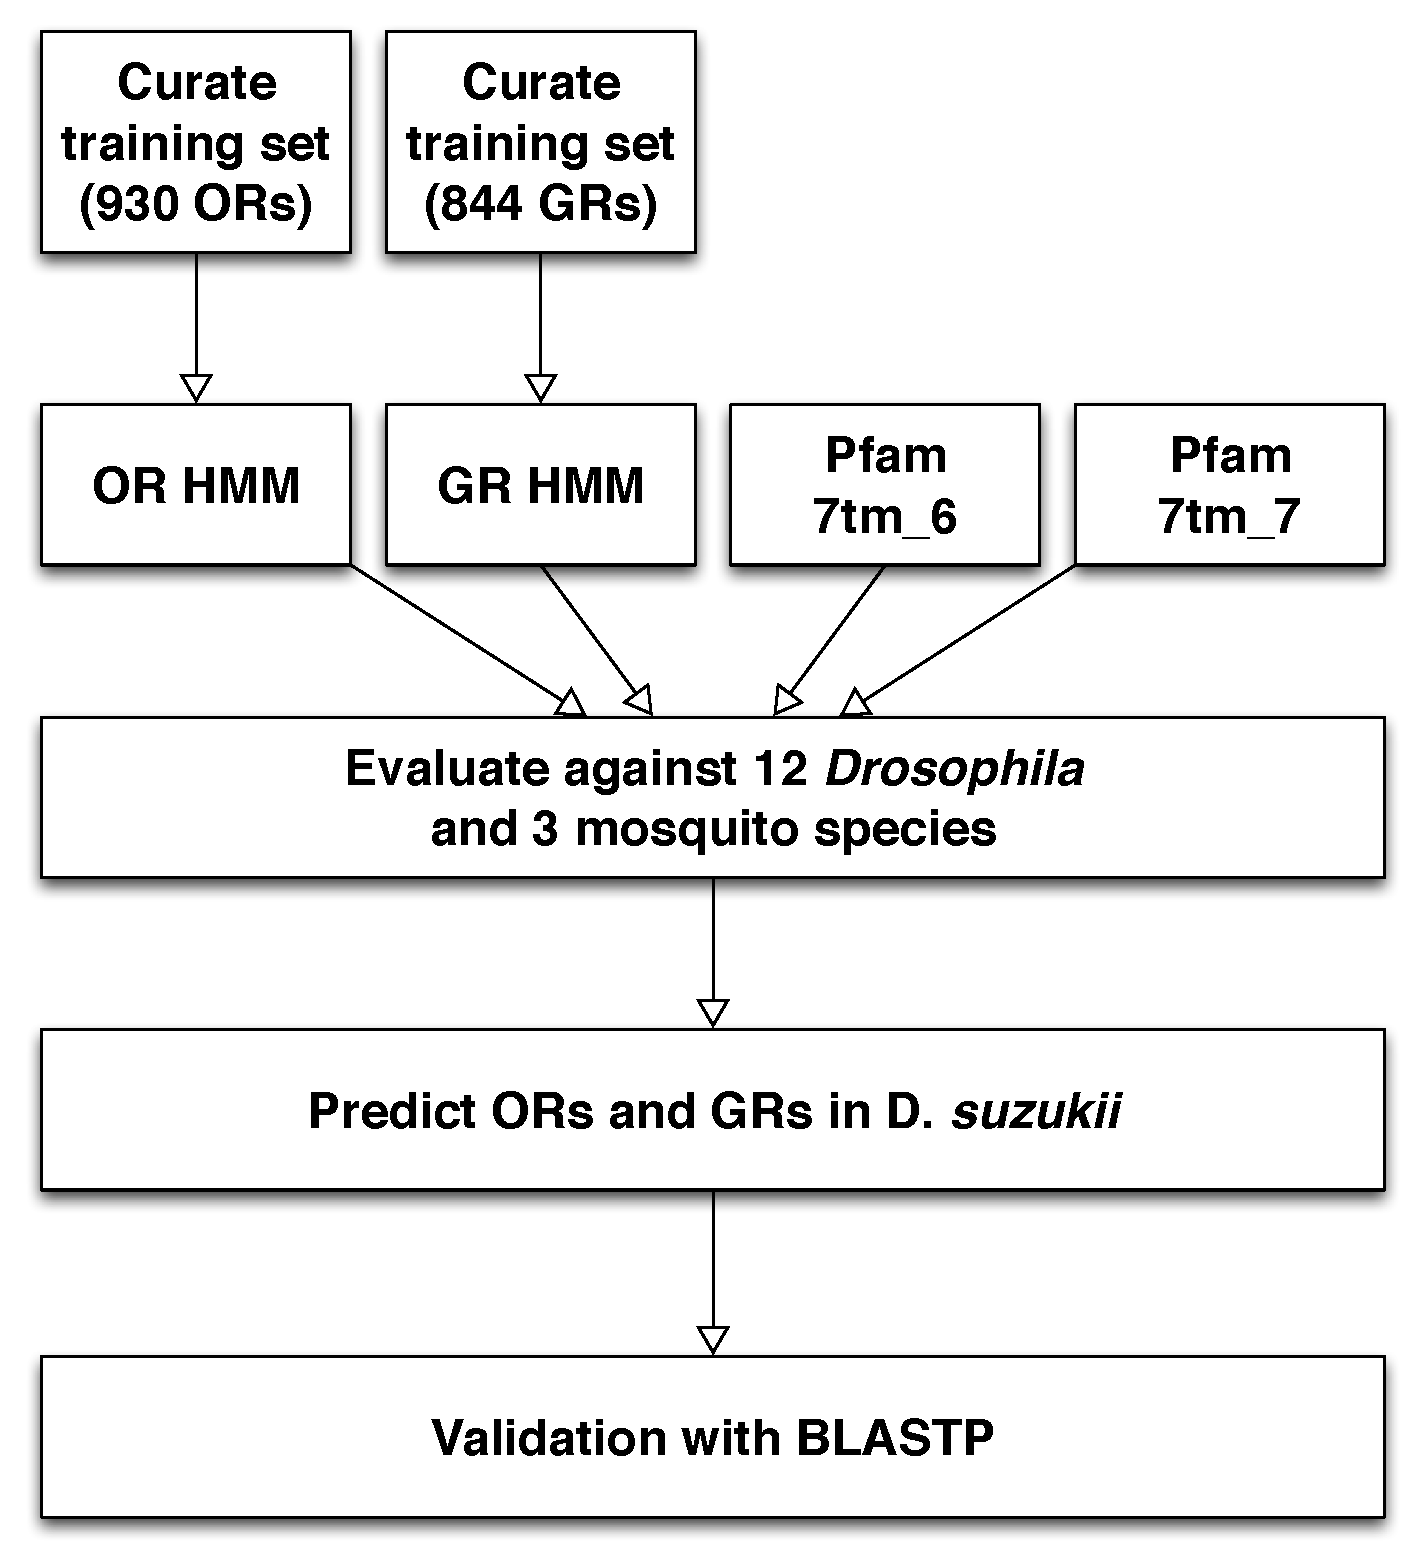
\includegraphics[width=0.7\textwidth]{figures/chemosensory/hmm_workflow}
  \caption{Workflow for HMM training, validation, and classification}
  \label{fig:chemosensory:hmm-workflow}
\end{figure}

\subsection{Results}

\subsubsection{Characterization of Insect Chemosensory Receptors}

\begin{figure}[H]
  \centering
  \begin{subfigure}[b]{0.45\textwidth}
    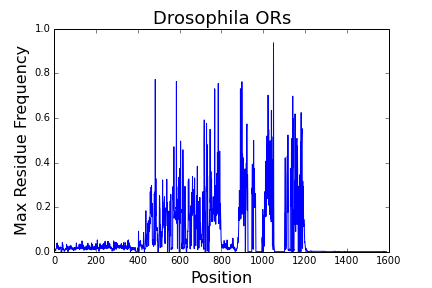
\includegraphics[width=\textwidth]{figures/chemosensory/drosophila_or_max_freq.png}
    \caption{Olfactory Receptors (930)}
    \label{fig:chemosensory:or-max-freq}
  \end{subfigure}
  ~
  \begin{subfigure}[b]{0.45\textwidth}
    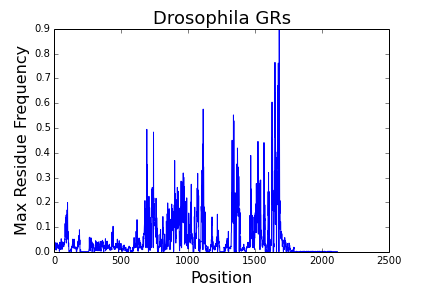
\includegraphics[width=\textwidth]{figures/chemosensory/drosophila_gr_max_freq.png}
    \caption{Gustatory Receptors (844)}
    \label{fig:chemosensory:gr-max-freq}
  \end{subfigure}
\label{fig:chemosensory:max-freq}
\caption{}
\end{figure}

\subsubsection{Comparing Approaches for Automated Identification}

\begin{table}[H]
  \centering
  \begin{tabular}{c c c c} \hline
  \emph{HMM} & \emph{Olfactory Receptors} & \emph{Gustatory Receptors} & \emph{Others} \\ \hline
  7tm\_6 & 881 & 15 & 223 \\ \hline
  OR & 928 & 68 & 297 \\ \hline
  7tm\_7 & 213 & 829 & 580 \\ \hline
  GR & 131 & 828 & 271 \\ \hline
  \end{tabular}
  \caption{Predicted Proteins from 12 \textit{Drosophila} and 3 mosquito species}
  \label{tab:chemosensory:hmm-validation}
\end{table}

\subsubsection{Identification \& Validation of \emph{D. suzukii} Chemosensory Receptors}

\begin{table}[H]
  \centering
  \begin{tabular}{c c c} \hline
  & \emph{Olfactory Receptors} & \emph{Gustatory Receptors} \\ \hline
  Predicted & 64 & 52 \\ \hline
  Validated & 56 & 45 \\ \hline 
  \end{tabular}
  \caption{Predicted and Validated Proteins \emph{D. suzukii}}
  \label{tab:chemosensory:suzukii-predictions}
\end{table}

\subsection{Discussion and Conclusion}